\subsection{Overview}
\subsubsection{Definition}
\subsubsection{Purpose}
\subsection{Importance in Modern Digital Exosystem}

\subsubsection{Evolution of User Behavior}
The digital landscape has seen a major evolution in user behavior, particularly in the way people interact with technology. In the early stages of the internet, user behavior was device-specific, primarily bounded to desktop computers. This era was characterized by more predictable online activities, with users typically accessing the internet from fixed locations and a small amount of different devices, which made user tracking relatively easy.

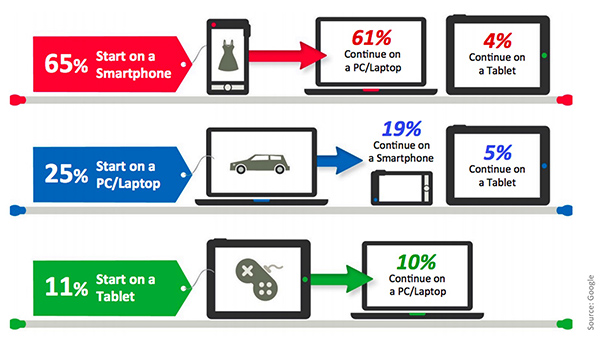
\includegraphics[width=0.95\textwidth]{./assets/google-cdt-stats.jpeg}

The invention of mobile technologies, especially smartphones changed online activities significantly and lead to a transformation in user behavior. Users began interacting with digital content across multiple platforms and often seamlessly switching between devices. For reference, Google published an interesting statistic, that shows more than 80 percent of all users switching their device during the user journey. Multi-platform interaction introduced a new level of complexity in understanding user behavior as users were no longer restricted to a single device.

Moreover, the rise of smart devices and the Internet of Things in the last years are the reason for  even more complex interactions between devices. Today, a wide network of connected devices are creating a diverse and complex digital footprint.

\subsubsection{Challenges in User Tracking}
Parallel to the evolution of users online behavior, the task of tracking users across multiple devices has become increasingly challenging. As there exists no universal login system or consistent identifiers across different websites, establishing a meaningful user profile from disparate device usage is really complex.

Privacy considerations make cross-device tracking even more complicated. With increasing sensitivity to data privacy and the introduction of strong regulations like the General Data Protection Regulation (GDPR) and the California Consumer Privacy Act (CCPA), tracking users across devices must navigate the line between effective data collection and respect for user privacy and consent.

The diversity of devices and platforms results in fragmented data sources, requiring advanced technological solutions for data integration and analysis. The need for algorithms and technologies is necessary to not only gather but also accurately interpret the large amount of data generated by multi-device usage.

Looking ahead, these challenges will even intensify with the continuous evolution of technology. The integration of artificial intelligence and machine learning will potentially lead to advancements in user tracking, but also brings additional complexities regarding privacy regulations. The task of user tracking demands innovative solutions that are adaptable, take privacy into account and are able of decoding increasingly complex device interactions.

\subsection{Techniques Employed in CDT}
\subsubsection{Deterministic Tracking}
\subsubsection{Probabilistic Tracking}
\subsubsection{Other Techniques}